\chapter{Základní problematika virtualizace síťových funkcí}
Jak již vyplývá z názvu, tak tato kapitola se zabývá základní analýzou a popisem problematiky spojené s oblastí virtuální síťových funkcí. 

Produkční vývoj v telekomunikačním průmyslu se tradičně řídil přísnými standardy kvůli stabilitě a kvalitě komunikace. Přestože tento model v minulosti fungoval, tak vedl nevyhnutelně k dlouhým produkčním cyklům, pomalému tempu vývoje a spoléhání se na proprietární či specializovaný hardware. S příchodem výrazné konkurence v komunikačních službách, od rychle postupujících organizací operujících ve velkém měřítku na veřejném internetu, podnítil poskytovatele služeb pro hledat nových způsobů, jak změnit dosavadní způsob produkčního vývoje.

Pro vyřešení toho problému bylo navrženo v publikacích \cite{NFV_paper2012} a \cite{NFV_paper2013} skupinou několika telekomunikačních provozovatelů řešení ve formě virtualizace síťových funkcí (network functions virtualization). Toto řešení má za cíl zlepšit následující aspekty provozu telekomunikačních sítí:

\begin{itemize}
\item Smíření investičních nákladů – snížení potřeby nákupu jednoúčelových hardwarových zařízení, možnost platby pouze za využité kapacity a snížení rizik přílišného předimenzování kapacit
\item Snížení provozních nákladů – snížení prostoru, napájení a požadavky na chlazení, zjednodušení správy a řízení síťových služeb
\item Urychlení Time-to-market – zkrácení doby pro nasazení nových síťových služeb, chopení se nových příležitosti na trhu, vyhovění potřebám zákazníka
\item Doručit agilitu a flexibilitu – možnost rychle škálovat (rozšiřovat nebo zmenšovat služby) dle měnících se požadavků od zákazníka. Podpora služeb, které mají být dodány pomocí softwaru na libovolném standardním serverovém hardwaru
\end{itemize}

Jak je uvedeno v \cite{NFVState} a \cite{NFVChalanges}, tak celá myšlenka je založena na tom, že dojde k separování softwarové funkcionality v síťových prvcích od proprietárního hardwaru, na kterém běží. To umožní se síťovými funkcemi zacházek jako s klasickými softwarovými aplikacemi, které mohou běžet na standardním komerčně dostupných serverech jenž organizace v současnosti používají. Tím bude zároveň umožněno flexibilní nasazování těchto síťových funkcí a jejich dynamický provisioning. Díky tomu, že jsou síťová funkce odděleny od hardwaru, tak je také možné jejich vhodnější umístění v topologii. To znamená dle požadavků na umístění mohou být nasazeny v datových centrech, síťových uzlech či přímo v uživatelově koncovém bodě. Hlavní koncept virtualizace síťových funkcí znázorňuje obrázek č. \ref{fig:vize_NFV}. 

\begin{figure}[h]
\begin{centering}
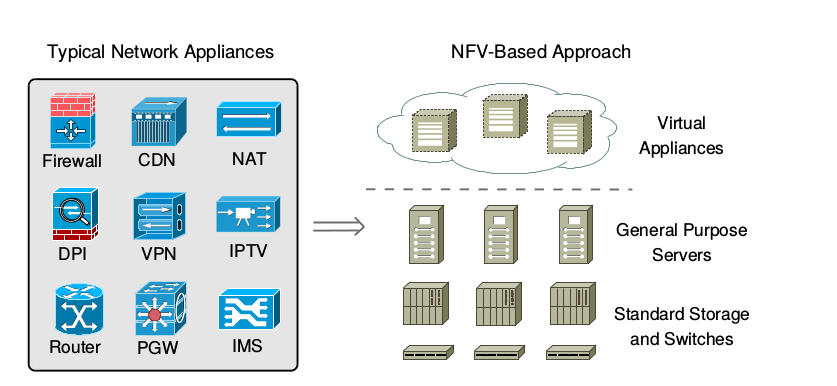
\includegraphics[scale=0.5]{images/vize_NFV}
\par\end{centering}
\caption{Koncept virtualizace síťových funkcí (NFV)\label{fig:vize_NFV}}
\end{figure}

Z zmínění stojí poznámka v \cite{NFVState}, kde je řečeno, že obecný koncept oddělení síťové funkce od hardwaru ještě nutně neznamená potřebu využití virtualizace. Protože budou síťové funkce dostupně jako software, tak mohou být nainstalovány a provozovány přímo na fyzickém stroji. Ovšem rozdíl je, že tento stroj již nebude speciální hardware, ale klasický server. Tento scénář může být do jisté míry použit při nasazovaní síťových funkcí v malém měřítku např. v uživatelských koncových bodech. Avšak pro plné využití všech výše zmíněných výhod, které jsou třeba ve velkých datových centrech, je třeba s použitím virtualizace počítat. To vše umocňuje fakt, že většina datových center v současnosti již využívá cloud computing.

Pro lepší pochopení a přehlednost celé této práce zde budou rozlišeny následující pojmy, se kterými se lze také setkat v odborné literatuře a které budou dále v této práci používány. 

\begin{itemize}
\item Síťová funkce (Network function - NF) - Toto je komponenta síťové infrastruktury, která má dobře definované funkční chování, jako například směrování, NAT, Load balancing, Intrusion detection, atd.
\item Virtuální síťové funkce (Virtual network function - VNF) - Je stejná jako NF, ale zde je funkčnost implementována pomocí softwaru a je nezávislá na hardwaru, na kterém běží.
\item Virtualizace síťových funkcí (Network Functions Virtualization - NFV) - Zde se jedná o označení celého konceptu či frameworku.
\end{itemize}

\section{NFV a Cloud Computing}

Cloud Computing a virtualizace obecně jsou hlavní technologie, které umožnily virtualizaci síťových funkcí. Z toho důvodu zde budou stručně představeny. 

Virtualizací obecně označujeme techniky, které umožňují k dostupným hardwarovým zdrojům přistupovat jiným způsobem, než jakým fyzicky existují. Je tomu díky softwaru, který tento hardware abstrahuje a vytvoří tím virtuální prostředí. Virtualizované prostředí se dá snadněji přizpůsobit potřebám uživatelů, případně skrýt pro uživatele nepodstatné detaily (jako např. rozmístění hardwarových prostředků). Tento software se nazývá hypervisor.\cite{VM_book}

Jak zmiňuje \cite{VM_architektura}, tak existují tyto dva základní typy hypervisorů:

\begin{itemize}
\item Typ 1 (Nativní) - Tento hypervisor běží přímo na fyzickém hardwaru. Tím umožňuje provozovat více operačních systému na jednom fyzickém stroji. Příkladem takového hypervisoru je VMware ESXi a XEN.
\item Typ 2 (Hostovaný) - Na rozdíl od předchozího případu tento typ hypervisoru běží v prostředí operačního systému. Příkladem je například KVM či Microsoft Hyper-V
\end{itemize}

\begin{figure}[h]
\begin{centering}
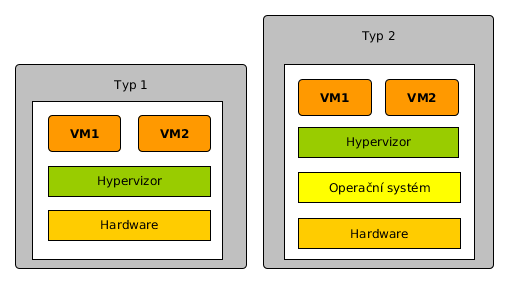
\includegraphics[scale=0.5]{images/virtualization}
\par\end{centering}
\caption{Schéma hypervisorů \label{fig:virtualization}}
\end{figure}

Obrázek \ref{fig:virtualization} zobrazuje schématický popis obou hypervisoru a jejich rozdíl. Problematika virtualizace je velice rozsáhlá a více informací o ní poskytují zdroje \cite{VM_book} a \cite{VM_architektura}.

Cloud Computing je nejpokročilejší formou virtualizace, kterou v poslední době začala provozovat většina větších organizací, jak ukazuje \cite{Cloud_adoption}. Cloud Computing má mnoho definic. V \cite{Cloud_book} je uvedeno, že se jedná o model, ve kterém lze uchovávat a poskytovat výpočetní zdroje, které jsou dostupné pomocí počítačové sítě s tím, že uživatelé k nim mohou přistupovat vzdáleně. Virtualizace síťových služeb umístěná v datových centrech je přímo svázaná s touto technologii. Z tohoto důvodu zde bude podrobněji popsán jejich vztah.

\subsection{Distribuční modely}

Dle \cite{CloudSurvey} lze cloudové služby lze rozdělit do 3 základních kategorii. V \cite{NFV_use_cases} jsou k těmto kategorii přiřazeny příklady užití z oblasti virtualizace síťových funkcí. 

\begin{itemize}
\item Infrastracture as a Service (IaaS) - Nejzákladnější  model  poskytování  cloudových  služeb. IaaS cloudové platformy nabízejí například výpočetní výkon, virtuální disky, blokové a souborové úložiště či virtuální sítě.  Poskytovatelé  IaaS  cloudových  platforem  poskytují tyto zdroje na vyžádání ze svých datových center. Toto je možné díky skupiny hypervisorů v rámci cloudu, které mohou provozovat velké množství virtuálních strojů  a  mají  schopnost  škálovat  poskytované  služby v  závislosti  na  měnících  se požadavcích přicházejících od zákazníků. Tento model může tedy sloužit i pro poskytnutí všech potřebných zdrojů celé infrastruktury pro virtualizaci síťových prvků, neboli Network Function Virtualization Infrastrakture as a Service. Zde má uživatel pod nejvíce možností, jak navrhnout a spravovat virtuální síťové funkce, protože vzásadě dokáže nasazovat i vlastně navržené síťové funkce a nejen ty, které mu poskytuje provozovatel cloudu.
\item Platform as a Service (PaaS) - V  modelu  Platforma  jako  služba  (PaaS)  hostují  poskytovatelé cloudových  služeb určitou počítačovou  platformu, kterou následně poskytují koncovým uživatelům přes Internet. Tato platforma většinou bývá prostředí nějakého operačního systému, prostředí  pro  běh  určitého programovacího  jazyka,  databáze  a  webový  server.  Vývojáři  aplikací tím pádem  mohou provozovat a případně vyvíjet svá softwarová řešení bez výrazných nákladů a složitého nákupu a konfiguraci potřebného hardwaru a softwaru. Některé PaaS platformy nastavuje výpočetní  a  úložné  prostředky  aplikace  automaticky  tak,  aby  odpovídala  aktuálním požadavkům aplikace bez nutnosti zásahu zákazníka. NVF v tomto modelu může nabízet síťové služby, které se mohou skládat z více virtuálních síťových funkcí, neboli Virtual Network Platform as a Service. Zde je poskytnuta uživately velká kontrola nad konfigurací a ovládáním celé platformy.
\item Software as a Servicec (SaaS) - V modelu SaaS provozují poskytovatelé cloudových služeb aplikační software v cloudu a uživatelé  k  tomuto  softwaru  přistupují  pomocí  klientského  software  (např.  webové prohlížeče). Uživatelé  cloudu tedy  nespravují infrastrukturu  ani platformu, kde aplikace běží.  Není  proto  třeba zde nic instalovat  a  spouštět  aplikace  na  vlastních  počítačích uživatele, což velmi zjednodušuje údržbu. Cloudové aplikace se liší od ostatních aplikací v možnostech  škálování, kterého  může  být  dosaženo  díky  distribuci  úkolů  na  více virtuálních strojů, a tím reagovat na měnící se poptávku. Tento proces je pro uživatele služby transparentní, uživatel vidí pouze jeden přístupový bod pro danou aplikaci. Do této kategorie služeb může patřit poskytování virtuálních síťových funkcí, která je pouze ve formě softwarové aplikace, neboli VNFaaS. Takovéto aplikace poskytují síťovou funkci pro síťové správce a uživatele nejčastěji v privatním cloudu. 
\end{itemize}

\subsection{Modely nasazení}

Existuje několik základních modelů nasazení cloud computingu resp. cloudových platforem, které uvádí \cite{CloudSurvey}. V \cite{NFV_use_cases} lze k nim opět najít určité příklady z oblasti virtualizace síťových funkcí.

\begin{itemize}
\item Privátní cloud - Privátní cloud je  infrastruktura  provozována  výhradně  v  rámci  jedné  organizace. Může být spravován interně nebo prostřednictvím třetí strany a hostování může být opět interní nebo externí.  Aby  mohl  podnik  využít  privátní  cloud,  musí  nejprve  navrhnout a uzpůsobit k tomuto účelu svoji stávající infrastrukturu, která musí být virtualizována.  Vlastní  přechod  vyvolává  řadu  bezpečnostních  otázek,  které  je třeba řešit, aby se zabránilo vážným zranitelnostem celého řešení. Privátní cloud je přesně ten typ modelu, kde lze najít využití pro virtualizaci síťových funkcí.
\item Veřejný cloud - Veřejné cloudové jsou cloudové služby, jako jsou aplikace, výpočetní výkon, úložiště a další, které jsou k dispozici široké  veřejnosti.  Služby  jsou  poskytovány  zdarma  nebo  podle modelu  platby  za  množství  použitých  služeb.  Je  zvykem,  že  veřejní  poskytovatelé cloudových  služeb,  jako  je  Amazon  AWS,  Microsoft  nebo  Google,  vlastní  a  provozují hardwarovou infrastrukturu a nabízejí k ní přístup pouze přes Internet. V tomto modelu není očekáváno využívání NFV.
\item Hybridní cloud - Hybridní  cloud je  spojení  dvou  nebo  více  cloudů  (soukromých,  komunitních  nebo veřejných),  které  zůstávají  samostatné,  ale  jsou  těsně  propojeny.  Toto  složení  rozšiřuje možnosti  nasazení  cloudových  služeb  a  tím  umožňuje  IT  organizacím  využít  veřejné cloudové prostředky k uspokojení dočasných potřeb. Tato schopnost umožňuje hybridním cloudům škálovat přes více nezávislých cloudů. V tomto modelu může být využito NFV především na straně soukromého cloudu.
\item Komunitní cloud - V rámci komunitního cloudu sdílí infrastrukturu cloudu několik organizací, které mají společné zájmy (bezpečnost, dodržování předpisů, působnost, atd.). Komunitní cloud může být spravován interně nebo prostřednictvím třetí strany. Náklady jsou rozloženy mezi méně uživatelů než na veřejném cloudu. V tomto modelu může být využito NVF, pokud se provozovatelé takovéhoto cloudu domluví. 
\end{itemize}


\section{NFV a SDN} \label{sub:SDN}

Softwarově definované sítě (SDN) je další z nových technologii, která se snaží vylepšit a automatizovat správu stávajících počítačových sítí. Dle \cite{SDN_clanek} jde o koncept, ve které je oddělena řídící logika (control plane) z jednotlivých routerů a switchů, které přeposílají traffic (data plane). Tím, že dojde k oddělení datové a řídící vrstvy, se routery a switche stanou pouze přeposílající data a veškerá řídí logika může být implementována v jednom logicky centrálním místě (SDN Controller). Z tohoto centrálního místa lze do jednotlivých routerů a switchů předávat instrukce pomocí aplikačních programovacích rozhraní (API). Samotný SDN Controller také obsahuje API, které mohou využívat aplikace a tím řídit, resp. programovat celou počítačovou síť. Obrázek č. \ref{fig:SDN} úkazuje jednoduché schéma softwarově definovaných sítí.

\begin{figure}[h]
\begin{centering}
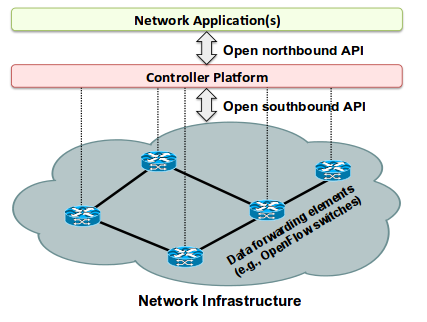
\includegraphics[scale=0.60]{images/SDN}
\par\end{centering}
\caption{Schéma SDN, převzato z \cite{SDN_clanek}\label{fig:SDN}}
\end{figure}

Přestože Softwarově definované sítě a virtualizace síťových funkcí jsou dvě různé technologie a koncepty, tak se navzájem se doplňují. Fakt, že SDN umožňuje programaticky ovládat počítačovou síť, lze využít pro poskytnutí programovatelné konektivity mezi jednotlivými virtuálními síťovými funkcemi. Naopak SDN může využít NFV tím, že implementuje potřebné síťové funkce jako software. Může tak virtualizovat SDN Controller, který tak může běžet na co nejvíhodnějším místě v datovém centru. Je vidět, že tyto dvě technologie se dobře doplňují, proto jsou často součástí jednoho řešení. \cite{SDN_book}

\section{Architektura NFV a VNF}

V předchozí sekci byla popsána myšlenka a motivace související s virtualizací síťových funkcí. Protože cílem této práce je navržení jednoduchého NFV frameworku, tak je nejprve nutné se seznámit s jeho obecnou architekturou. V této práci se bude vycházet z referenční architektury NVF \cite{NFV_architektura}, která byla navržena organizací ETSI. Jedná se pouze o funkční návrh bez náznaků konkrétní implementace. Od této skupiny existují i podrobnější návrhy jednotlivých částí celého NFV frameworku, které v této práci budou také popsány v příslušných kapitolách.

\begin{figure}[h]
\begin{centering}
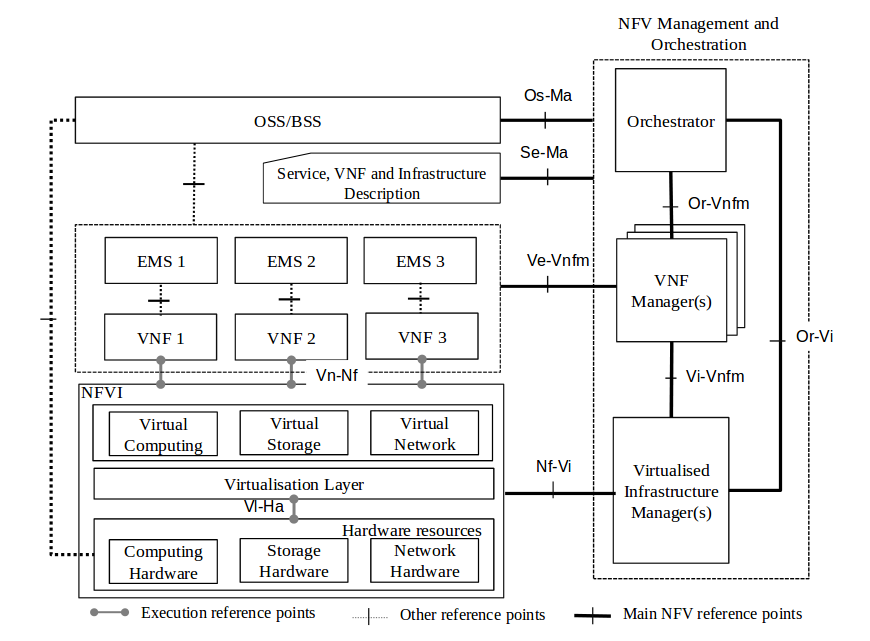
\includegraphics[scale=0.5]{images/NFV_architektura}
\par\end{centering}
\caption{NFV architektura, převzato z \cite{NFV_architektura}\label{fig:NFV_architektura}}
\end{figure}

Jak je vidět na obrázku č. \ref{fig:NFV_architektura}, tak celá architektura se dá rozdělit na tyto 3 hlavní části:

\begin{itemize}
\item Infrastruktura virtualizace síťových funkcí (NFVI) - Jsou všechny softwarové a hardwarové zdroje potřebné k vytvoření prostředí, ve které mohou být jednotlivé VNF být nasazeny. Tato infrastruktura může být velice rozsáhlá, proto je její součástí i síť poskytující konektivitu mezi vzdálenými lokacemi infrastruktury.\cite{NFV_terminology}
\item Virtualizované síťové funkce (VNFs) - Jsou softwarové implementace síťových funkcí, jako je např. NAT a routing. které mohou být nasazeny na NFV infrastruktuře.
\item Management a orchestrace NFV (NFV-MANO) - zde se jedná o řízení softwarových a hardwarových zdrojů v celé infrastruktuře NFV a životního cyklu jednotlivých virtuálních síťových funkcí. Tato část se tedy zaměřuje na řízení a správu všech úloh související v virtualizací v NFV frameworku. \cite{NFV_terminology}
\end{itemize}

Tyto funkční bloky se ještě dále dělí, proto dále v této práci budou tyto jednotlivé části popsány podrobněji a současně k nim budou uvedeny různé možnosti řešení.

\subsection{Infrastruktura NFV}

Ve zdroji \cite{NFV_infrastructure}, který detailně popisuje infrastrukturu pro virtualizaci síťových funkcí (NFVI), je uvedeno, že je v ní sdružení všech základních zdrojů potřebných pro běh virtuálních síťových funkcí (VNF). Z tohoto důvodu sem patří veškerý hardware. Do NFVI také patří některé softwarové komponenty, které jsou společné mnoho VNF a poskytují funkcionalitu potřebnou pro podporu nasazení, propojení či managementu VNF. Celou infrastrukturu může tvořit jeden či více strojů, které mají tyto potřebné funkce. Tyto stroje také mohou být umístěny v různých spolu spojených lokacích. 

Pro zjednodušení lze celou NFV infrastrukturu rozdělit do 3 následujících domén:

\begin{itemize}
\item Compute Domain - Do této domény patří veškeré hardwarové zdroje jako jsou servery, úložiště a komponenty, které tyto zdroje obsahují, např. procesory, pevné disky, síťové karty, atd. Zároveň je zde řešen návrh fyzické topologie. \cite{NFV_compute}
\item Hypervisor Domain - Toto je doména, které představuje softwarové prostředí abstrahující hardware v compute doméně a poskytuje je jako virtuální zdroje. Tyto zdroje následně mohou využívat virtuální síťové funkce. \cite{NFV_hypervisor}
\item Infrastructure Network Domain - V této doméně je řešeno veškeré propojení výše zmíněných domén. Tedy fyzické i virtuální infrastruktury.\cite{NFV_network}
\end{itemize}

Funkci obsaženou v jednotlivých doménách znázorňuje obrázek č. \ref{fig:infrastruktura}. Více informací na tuto problematiku lze nalézt v \cite{NFV_infrastructure} a ve zdrojích uvedených u každé domény. 

\begin{figure}[h]
\begin{centering}
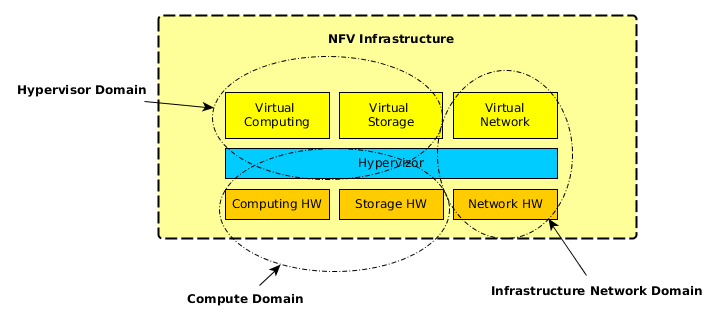
\includegraphics[scale=0.65]{images/infrastruktura}
\par\end{centering}
\caption{Schéma NFV infrastruktury\label{fig:infrastruktura}}
\end{figure}

Dá se říci, že návrh infrastruktury pro NVF je podobný jako pro návrh infrastruktury pro cloud computing platformu. Měl by se tedy skládat z generických a komerčně vysoce dostupných serverů, které by měli být zapojeny do switche a tím by měla být zajištěna konektivita. Na tyto servery je následně nasazen jeden z dostupných hypervisorů. Výběr správného hypervisoru, které jsou v současné době dostupné na trhu, je hlavní podmínka správného a funkčního návrhu této části NFV frameworku. Přehled hypervisorů je uveden v kapitole \ref{sub:Hypervisor}. V produkčním prostředí by součástí řešení bylo samozřejmě řešení síťového návrhu. Tato práce však má sloužit pouze jako ukázka a z tohoto důvodu zde nebude síťový návrh zmíněn.

\subsection{Virtuální síťová funkce}

Virtuální síťová funkce (VNF) je dle \cite{NFV_VNF} určitá síťová funkce, která běží na NVF infrastruktuře a je zárověň NVF frameworkem řízena a spravována. Zároveň musí mít dobře definované rozhraní k ostatním síťovým funkcím, k VNF Managerovi a měla by obsahovat management rozhraní či port. 

Síťové funkce jsou tedy obvykle realizovány pomocí virtuálních strojů či dnes již často používaných konteinerů. Závisí na použité virtualizační platformě. Jedna VNF může být být obsažena v jednom virtuálním stroji nebo může být roztažena přes více virtuálních strojů. 

Na obrázku č. \ref{fig:VNF} je vidět jednoduché schéma virtuální síťové funkce. Celý životní cyklus VNF, což je vytvoření, spuštění, zastavení, smazání a škálování, řídí VNF Manager, který je součástí NVF managementu a orchestrace. Současně je možné dynamicky změnit aktuální konfiguraci pomocí Entity manageru (EM) přes management interface. EM může spravovat více VNF nebo právě jednu. Vnitřní struktura celé instance může být tvořena více komponentami (VNFC), které spolu mohou být navzájem provázány. Toto provázání však nemusí být viditelné zvenčí.

\begin{figure}[h]
\begin{centering}
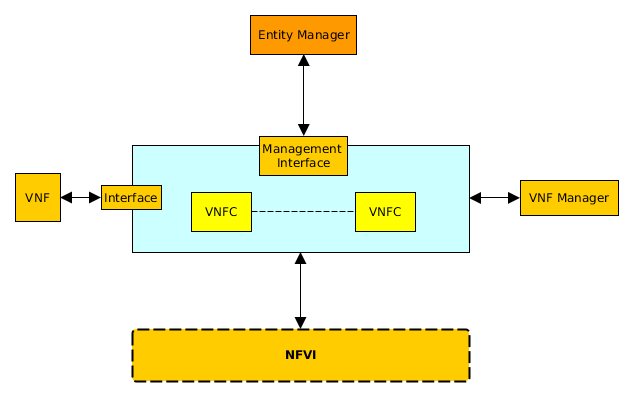
\includegraphics[scale=0.67]{images/VNF}
\par\end{centering}
\caption{Schéma virtuální síťové funkce\label{fig:VNF}}
\end{figure}

\subsubsection{Service Chaining}

Jednou z výhod NFV je možnost využít Service Chaining. Service chaining je ve skutečnosti součást SDN, které bylo zmíněno v kapitole \ref{sub:SDN}. Jde o princip jakým lze dynamicky pospojovat jednotlivé VNF. \cite{SDN_book}

Service chaining není ve skutečnosti nic nového. V klasických počítačových sítích je používán také, ale pomocí fyzických síťových prvků. Jedná se zjednodušeně o způsob zapojení mezi jednotlivými síťovými prvky (či VNF) a způsob, jakým na sebe navazují. Příklad takového zapojení je vidět na obrázku č. \ref{fig:service_chaining}. Zde se provozovatel sítě rozhodl, že odchozí data z klientských stanic musí jít přes firewall, IDS a nakonec přes NAT do Internetu. Příchozí data mají logicky obrácené pořadí. Toto zapojení funguje dobře pro síť, kde není třeba rozlišovat cestu jakou proudí data jednotlivých uživatelských stanic. Ale není to optimální řešení pro sítě s více uživateli, kde každý požaduje jinou síťovou funkci. Potřeba jednotlivých síťových služeb se samozřejmě může v čase měnit. Příklad takové sítě lze nalézt ve většině datových center. 

\begin{figure}[h]
\begin{centering}
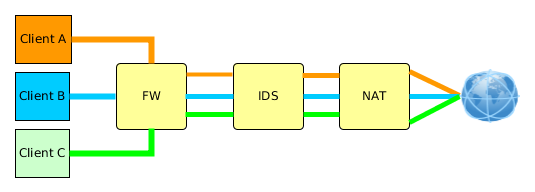
\includegraphics[scale=0.55]{images/service_chaining}
\par\end{centering}
\caption{Ukázka klasického service chainigu pomocí fyzických síťových prvků\label{fig:service_chaining}}
\end{figure}

Zde tedy přichází na řadu VNF spolu s SDN. Protože jednotlivé VNF existují jako virtuální stroje, tak mohou být dynamicky nasazovány dle aktuálním požadavků jednotlivých klientů a pomocí SDN mohou být tyto VM dynamicky pospojovány. Obrázek č. \ref{fig:service_chaining_new} ukazuje schéma zapojení, kde každý klient může mít jinou požadovanou cestu do internetu. Je možná i varianta, kde každý klient má své vlastní VNF s jinou konfigurací.

\begin{figure}[h]
\begin{centering}
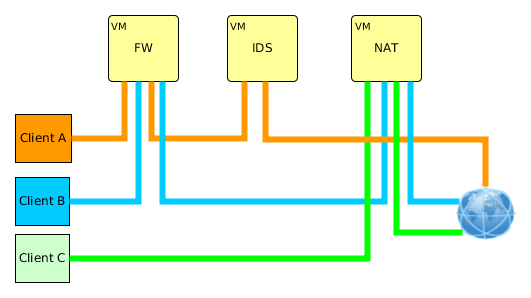
\includegraphics[scale=0.55]{images/service_chaining_new}
\par\end{centering}
\caption{Ukázka VNF service chainigu\label{fig:service_chaining_new}}
\end{figure}

\subsection{Management a orchestrace NFV}

Management a orchestrace virtualizace síťových funkcí (NFV MANO) je nejdůležitější celého NFV frameworku. 

\begin{figure}[h]
\begin{centering}
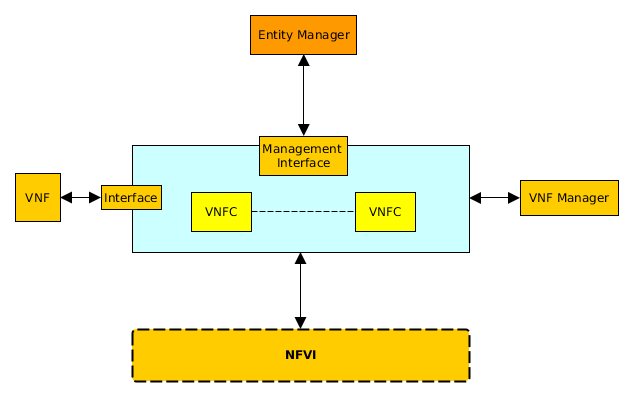
\includegraphics[scale=0.65]{images/VNF}
\par\end{centering}
\caption{Schéma NFV MANO\label{fig:VNF}}
\end{figure}


	\subsubsection{Orchestrator}

	\subsubsection{VNF manager}

	\subsubsection{Virtualised Infrastructure Manager}



\section{Možné technologie pro řešení}

\subsection{Hypervisory} \label{sub:Hypervisor}

KVM, Hyper-V, VMware ESXi


\subsection{VNF}

Juniper vSRX, Fortigate VM, PFSense, Cisco ASAv, Vyatta, M0n0wall, OpenStack Neutron HAproxy

\subsection{Cloud platforma}

OpenStack, VMware

\subsection{SDN}

OpenContrail, VMware






